\documentclass[10pt]{article}
\usepackage{bm, url, graphicx, amsmath}
\nonstopmode

\title{DiRAC Benchmarks}
\author{...}

\begin{document}

\maketitle

\section{DiAL: Data Intensive at Leicester}

\subsection{Overview{\footnote{see \url{https://www2.le.ac.uk/offices/itservices/ithelp/services/hpc/dirac/about}}}
}

The University of Leicester hosts one of five High Performance Computing (HPC) systems that forms part of the DiRAC service. The focus of the service is to support data intensive science problems in Theoretical Astrophysics and Particle Physics. The DIaL service provides:

\begin{itemize}
	\item 400 dual-socket nodes with 36 2.3 GHz intel skylake cores, 192 GB RAM per node.
	\item 3 large memory nodes: 36 skylake cores, 1.5TB RAM per node.
	\item 1 large memory node with 144 skylake 3GHz cores, 6 TB RAM, supporting larger shared memory codes.
	\item EDR Infiniband Interconnect (2:1 blocking)
	\item 3.3 TB of Lustre parallel storage, supporting over 40GB/s read/write.
	\item 100 GB NVMEoFC storage - experimental data intensive file store with a theoretical peak read/write of 50GB/s.
	\item All nodes run linux CentOS 7 or RHEL 7
\end{itemize}

\clearpage
\subsection{Benchmarks}

\subsubsection{Ramses}
TODO

\begin{figure*}[h!]
	\centering
	\includegraphics[width=0.7\textwidth]{Ramses_strong.pdf}
	\vspace{0.1cm}
	\hrule
	\vspace{0.1cm}
	\caption{.}
	\label{fig::ramses_ss}
\end{figure*}


\begin{figure*}[h!]
	\centering
	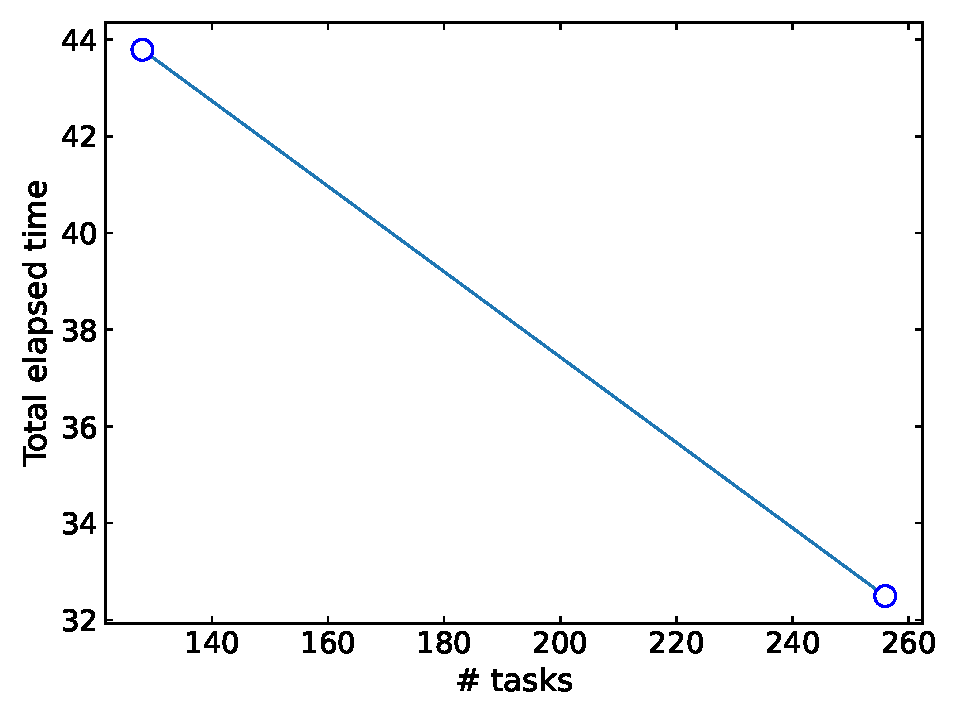
\includegraphics[width=0.7\textwidth]{Ramses_weak.pdf}
	\vspace{0.1cm}
	\hrule
	\vspace{0.1cm}
	\caption{.}
	\label{fig::ramses_ws}
\end{figure*}


\clearpage
\subsubsection{Sphng}
TODO

\begin{figure*}[h!]
	\centering
	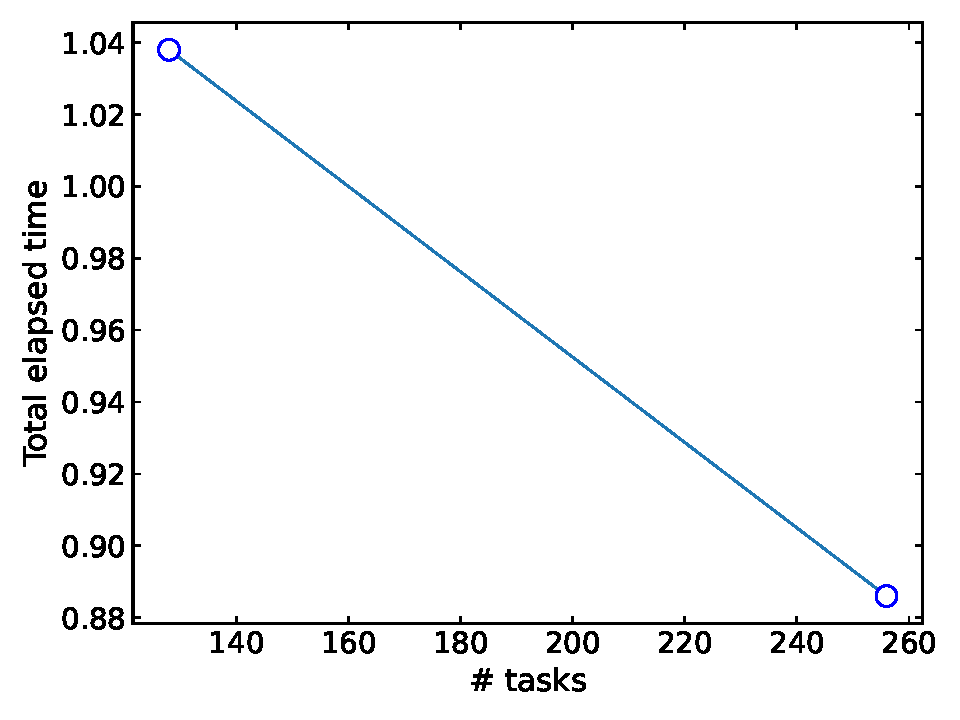
\includegraphics[width=0.7\textwidth]{Sphng_strong.pdf}
	\vspace{0.1cm}
	\hrule
	\vspace{0.1cm}
	\caption{.}
	\label{fig::sphng_ss}
\end{figure*}


\begin{figure*}[h!]
	\centering
	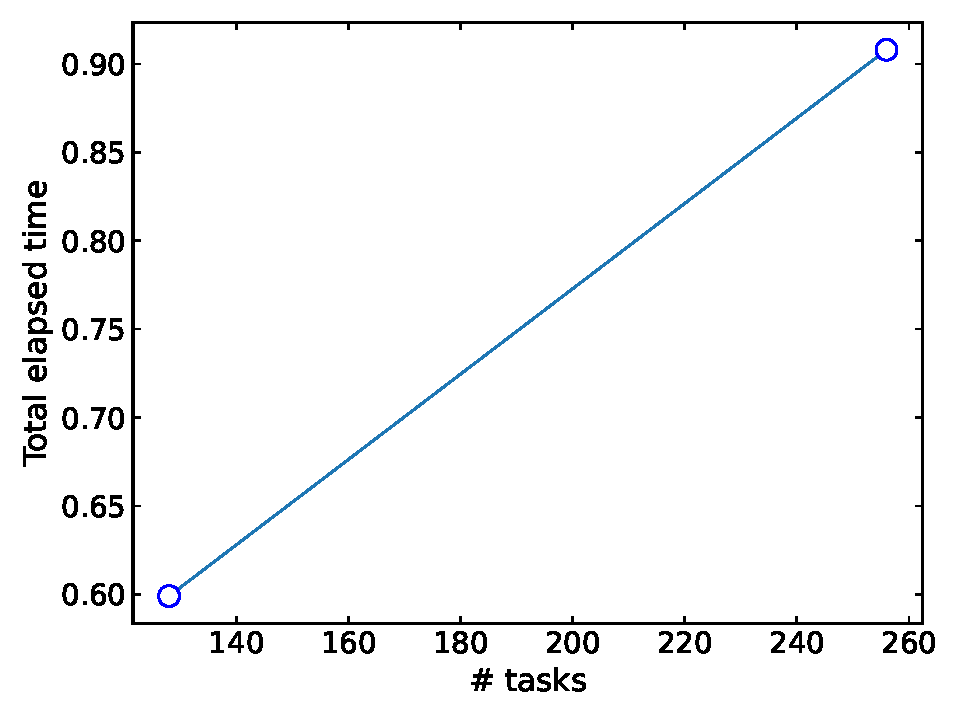
\includegraphics[width=0.7\textwidth]{Sphng_weak.pdf}
	\vspace{0.1cm}
	\hrule
	\vspace{0.1cm}
	\caption{.}
	\label{fig::sphng_ws}
\end{figure*}


\clearpage
\subsubsection{Trove}
TODO


\clearpage
\subsection{Summary}

TODO



\end{document}